\section{End-to-End Learning for Robot Control}

  End-to-end refers to a robot learning approach where the robot determines certain \textbf{policies}from raw inputs from the action space. The action space can include anything that we think the robot may benefit form knowing. This means the robot learns to map sensory inputs directly to motor commands, bypassing the need for intermediate steps such as feature extraction or state estimation. This approach leverages deep learning techniques \cite{Schmidhuber2015nn}, particularly convolutional neural networks (CNNs) and recurrent neural networks (RNNs), to process high-dimensional sensory data and generate appropriate actions. Which can then be used in techniques like Reinforcement Learning \ref{sec:rl} or Imitation Learning \ref{sec:il}. Therefore, recent advancements in machine learning technologies has also reshaped the field of robotics and helps move it forward \cite{Pierson18082017,newbury2023graspSynthReview,liu2021DRLminireview}.

  \begin{figure}[h]
    \centering
    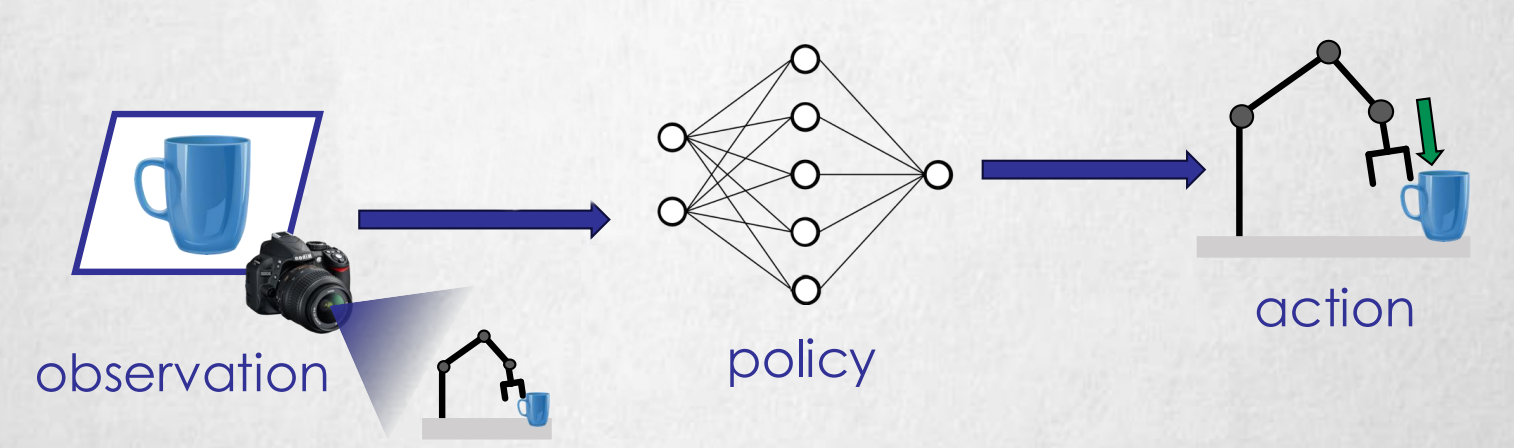
\includegraphics[width=0.6\textwidth]{assets/intro/endtoend.png}
    \caption{Diagram showcasing simple end to end learning ideas, modified from \cite{johns2024}}\label{fig:end2end}
  \end{figure}

  This contrasts with the classical approaches. Classical robotics involves separating the behaviour of a robot into smaller tasks, where each task is managed by a distinct module and the system is functional when the pipeline comes together. Although good at precisely executing repetitive tasks, this approach requires complex and often handcrafted solutions for each module. This can lead to difficulties in scaling and adapting to new tasks or environments. 
  
  Therefore, the cutting-edge research in robotics concerns end-to-end systems in making multi-modal robots, which can be tuned for specific tasks if needed, using their capabilities of complex decision-making withing the given environments.

% Math Foundations
\section{Mathematical Foundations}

  In scenarios involving autonomous acting, the capability of a an robot to reason and navigate complex problems or dynamic environments plays a central role. So in any RL system the agent must make a sequence of decisions that impact later outcomes. Markov Decision Processes (MDPs) provide a mathematical framework for modelling decisions in environments where the probabilistic outcomes are influenced by actions of such an agent. A formally defined MDP will have the following parts:

\subsection{Markov Decision Processes}\label{sec:mdp}
  \subsubsection{State, S}
    The system must be able to process all different configurations of the environment. So the state will encapsulate the surroundings through raw sensory inputs (e.g. images, force sensors) in a high-level representation and will capture all relevant information available \cite{Sutton1998} which might be needed to make an informed decision at a particular time step.

  \subsubsection{The Markov Property}
    A state $S_t$ is \emph{Markov} if and only if:
    \[
      \mathbb{P} \left[S_{t+1} \mid S_t\right] = \mathbb{P}\left[ S_{t+1} \mid S_1, \ldots, S_t\right]
    \]

   % \todo{maybe make this a lemma type table??}
    This property ensures that all relevant information from the history is captured within the state. So once the state is knows the past states can be discarded. Making the current state a sufficient statistic for the future \cite{silver2015}.

  \subsubsection{State Transition Matrix, P}
    This matrix defines the transition probabilities from all states $s$ to all successor states $s'$, so:
    
    \[ P_{ss'} = \mathbb{P} \left[S_{t+1} = s'  \mid S_t = s\right]\] 
    and 
    
    \[ P =
    \begin{bmatrix}
      P_{11} & \cdots & P_{1n} \\ 
      \vdots & & \vdots\\
      P_{n1} & \cdots & P_{nn}
    \end{bmatrix}
    \]
    where each row of the matrix sums up to 1, due to the nature of probabilities. A tuple of a set of states and a transition matrix/function \(\langle S, P \rangle\) make up a \textbf{Markov Process} (or Markov Chain)

  \subsubsection{Actions, A}
    This is the set of all possible actions that are available to the robot in each state. Depending on the context of the task, actions can be discrete or continuous. Related back to robotics: state-based systems like RL for solving games will be discrete, while the movement of a physical robot is generally a continuous action.

  \subsubsection{Reward Function, R}
    A scalar feedback signal which ensures that the agent's learning is based on steps it is taking over time, so $R_t$ is how well the agent is doing at step $t$. It is defined as:

    \[R_s = \mathbb{E} \left[R_{t+1} \mid S_t = s\right]\]
    
    This allows the robot to eventually converge to a solution that maximises the cumulative rewards (the \emph{returns}) for the actions it has taken. 
  
  \subsubsection{Discount Factor, $\gamma$}
    Mechanism to control the importance of future rewards. Sampled as: \(\gamma \in \left[0, 1\right]\), means that immediate reward is prioritised while reward form longer sequence of actions will decay in priority. Helping avoid infinite cycles in Markov Chains.

    Combining the reward function and the discount factor we can define the \emph{return}, $G_t$ as the total discounted reward from time-step $t$:

    \[ 
    \begin{aligned}
      G_t &= R_{t+1} + \gamma R_{t+2} + \ldots \\ 
      &= \sum_{k=0}^{\inf}\gamma^k R_{t+k+1} 
    \end{aligned}
    \]
    
    Therefore, a \emph{Markov Decision Process} is a tuple \(\langle S, A, P, R, \gamma \rangle\) as the parts are defined above.
    
    
  \subsubsection{Policy, $\pi$}
    The higher-level goal of any RL system is to learn an optimal policy \(\pi \left( a \mid s\right) = \mathbb{P} \left[A_t = a \mid S_t = s\right]\) which aims to maximise the return. Policies fully define the behaviour of the agent. As seen by the function's type \(\pi: S \rightarrow A \); they only depend on the current state and are time independent \( A_t \sim \pi\left( \cdot \mid S_t\right), \forall t > 0 \).
    
  \subsubsection{Value Functions}
    On top of these we define two value function, \emph{state-value}: the expected return starting from state $s$, and then following policy $\pi$:

    \[ v_\pi \left(s\right) = \mathbb{E} = \left[G_t \mid S_t = s\right]\]

    and the \emph{action-value} function, which is the expected return starting from state $s$, taking action $a$, and then continuing a policy $\pi$:

    \[ q_\pi \left(s, a\right) = \mathbb{E} \left[ G_t \mid S_t = s, A_t = a\right]\]


    while the optimal versions can be defined as:
    \[v_* \left(s\right) = \underset{\pi}{\max} \ v_\pi \left(s\right)\]

    \[q_* \left(s, a\right) = \underset{\pi}{\max} \ q_\pi \left(s, a\right)\]
    
    The optimal means the best possible performance can be achieved in the MDP and it can be considered ``solved'' once we find these optimal functions. Solutions to these will help estimate a mapping for a robot to its best-case movement within its current state.


    

% Reinforcement Learning
\section{Reinforcement Learning (RL)}
  One of the tried and tested methods of end-to-end learning approaches is a branch under machine learning called \emph{Reinforcement Learning (RL)}. \todo{is it a branch under machine learning?}
  \missingfigure{add the classic agent state reward action diagram}

  RL's main focus is training robots, which are called \emph{agents} in making decisions by interacting with the environment. The key objective is to teach a \emph{policy} to the agent that maximises the overall reward -usually defined by the task and involves a \emph{teacher}. The agent will explore, the possibly actions it can take through trail and error, while learning from the feedback given to it by the reward signal and its environment.

  One of the differentiating factors of RL from classical machine learning paradigms is that the feedback is not instantaneous and sequences of decisions influence the subsequent data and signals given to agent \cite{silver2015}.

  \subsection{Mathematical Foundations}

  In scenarios involving autonomous acting, the capability of a an robot to reason and navigate complex problems or dynamic environments plays a central role. So in any RL system the agent must make a sequence of decisions that impact later outcomes. Markov Decision Processes (MDPs) provide a mathematical framework for modelling decisions in environments where the probabilistic outcomes are influenced by actions of such an agent. A formally defined MDP will have the following parts \cite{silver2015}:

\subsection{Markov Decision Processes}
  \subsubsection{State, S}
    The system must be able to process all different configurations of the environment. So the state will encapsulate the surroundings through raw sensory inputs (e.g. images, force sensors) in a high-level representation and will capture all relevant information available \cite{Sutton1998} which might be needed to make an informed decision at a particular time step.

  \subsubsection{The Markov Property}
    A state $S_t$ is \emph{Markov} if and only if:
    \[
      \mathbb{P} \left[S_{t+1} \mid S_t\right] = \mathbb{P}\left[ S_{t+1} \mid S_1, \ldots, S_t\right]
    \]

   % \todo{maybe make this a lemma type table??}
    This property ensures that all relevant information from the history is captured within the state. So once the state is knows the past states can be discarded. Making the current state a sufficient statistic for the future \cite{silver2015}.

  \subsubsection{State Transition Matrix, P}
    This matrix defines the transition probabilities from all states $s$ to all successor states $s'$, so:
    
    \[ P_{ss'} = \mathbb{P} \left[S_{t+1} = s'  \mid S_t = s\right]\] 
    and 
    
    \[ P =
    \begin{bmatrix}
      P_{11} & \cdots & P_{1n} \\ 
      \vdots & & \vdots\\
      P_{n1} & \cdots & P_{nn}
    \end{bmatrix}
    \]
    where each row of the matrix sums up to 1, due to the nature of probabilities. A tuple of a set of states and a transition matrix/function \(\llangle S, P \rrangle\) make up a \textbf{Markov Process} (or Markov Chain)

  \subsubsection{Actions, A}
    This is the set of all possible actions that are available to the robot in each state. Depending on the context of the task, actions can be discrete or continuous.

  \subsubsection{Reward Function, R}
    This is the scalar feedback signal. It ensures that the agent's learning is based on steps it is taking over time, so $R_t$ is how well the agent is doing at step $t$. It is defined as:

    \[R_s = \mathbb{E} \left[R_{t+1} \mid S_t = s\right]\]
    
    This allows the robot to eventually converge to a solution that maximises the cumulative rewards (the \emph{returns}) for the actions it has taken. 
  
  \subsubsection{Discount Factor, $\gamma$}
    This is mechanism to control the importance of future rewards. Sampled as: \(\gamma \in \left[0, 1\right]\), means that immediate reward is prioritised and while reward form longer sequence of actions decays, avoiding infinite cycles in Markov Chains.

    Combining the reward function and the discount factor we can defined the \emph{return}, $G_t$ as the total discounted reward from time-step $t$:

    \[ 
    \begin{aligned}
      G_t &= R_{t+1} + \gamma R_{t+2} + \ldots \\ 
      &= \sum_{k=0}^{\inf}\gamma^k R_{t+k+1} 
    \end{aligned}
    \]
    
    Therefore, a \emph{Markov Decision Process} is a tuple \(\langle S, A, P, R, \gamma \rangle\) as the parts are defined above.
    
    
  \subsubsection{Policy, $\pi$}
    The higher-level goal of any RL system is to learn an optimal policy \(\pi \left( a \mid s\right) = \mathbb{P} \left[A_t = a \mid S_t = s\right]\) which aims to maximise the return. Policies fully define the behaviour of the agent. As seen by the function's type \(\pi: S \rightarrow A \) they only depend on the current state and are time independent \( A_t \sim \pi\left( \cdot \mid S_t\right), \forall t > 0 \)
    
  \subsubsection{Value Functions}
    On top of these we define two value function, \emph{state-value}: the expected return starting from state $s$, and then following policy $\pi$:

    \[ v_\pi \left(s\right) = \mathbb{E} = \left[G_t \mid S_t = s\right]\]

    and the \emph{action-value} function, which is the expected return starting from state $s$, taking action $a$, and then continuing a policy $\pi$:

    \[ q_\pi \left(s, a\right) = \mathbb{E} \left[ G_t \mid S_t = s, A_t = a\right]\]


    while the optimal versions can be defined as:
    \[v_* \left(s\right) = \underset{\pi}{\max} \ v_\pi \left(s\right)\]

    \[q_* \left(s, a\right) = \underset{\pi}{\max} \ q_\pi \left(s, a\right)\]
    
    The optimal means the best possible performance can be achieved in the MDP and it can be considered ``solved'' once we find these optimal functions.

    \todo{should I define the bellman function?}

    \subsection{Exploration and Exploitation}
    \todo{this is left for tmr man, I had enough gotta finish the model flavours}

\section{RL in Practice}
  Reinforcement learning, can be used to train a variety of agents that is not limited by physical robots. It can learn to play video-games \cite{comi2018}, automation tasks \cite{}, in natural language processing \cite{paulus2017deepreinforcedmodelabstractive}, applications  in healthcare (where RL is categorised as dynamic treatment regimes) for use in chronic diseases or critical care \cite{yu2020reinforcementlearninghealthcaresurvey} and lastly -most importantly for us- learning movement behaviours for robots \cite{}.
  \todo{add more sources and citations}
  
  A fundamental challenge in utilising RL is the constant act of balancing \textbf{exploration} and \textbf{exploration}. A trade-off must be made in the chosen model \todo{model might not be the right word here as it hints at model-based?}
  \begin{enumerate}
    \item \textbf{Exploration:}
    This is when the agent decides to \emph{explore} new actions that might potentially lead to better long-term outcomes. An issue this can cause is that the time it takes to explore all possibilities might not be feasible. But crucial to utilise in in problems with sparse reward models \cite{}
    \item \textbf{Exploitation:}
    When the agent prioritises short-term, immediate rewards by exploiting its current knowledge. For example, taking an agent playing a video game; if a high score was found the agent might be unaware that a higher score can be achieved with a different set of moves. 
  \end{enumerate}

  The trade-offs must be balanced between the two in any RL algorithm or model while considered sampling efficiencies and ease of training \cite{liu2019simpleexplorationsampleefficient}. To relate it back to a robotics example, too much exploration might lead to inefficient training and instability; while too much reliance on exploitation might lead to suboptimal behaviours in the movement of a robot executing a task. 

  Some common strategies are:
  \begin{itemize}
    \item $\epsilon$-Greedy:
    \item Decay $\epsilon$-Greedy:
    \item Upper Confidence Bound (UCB):
    \item Thompson Sampling
    \item Intrinsic Motivation (Curiosity-Driven Exploration):
    \todo{find sources and confirm and give quick details about pros/cons?}
  \end{itemize}
  
  Along with this widespread use and elemental challenges, comes differing methods of utilising the RL framework. The likes of which can be broadly classified into two types: \textbf{Model-Based} and \textbf{Model-Free}.
  
  \subsection{Model-Based RL}
  Model based approaches involve methods of creating an internal model and representation of the state the agent is interacting with. It usually involves two main steps: learning the dynamics of the model, then planning and learning within it \cite{MAL-086}. These models have underlying principals of the Markov Decision Process.
  \todo{link to markov decision process}

  Main power of this approach comes from its simulated core. As fewer real interactions can allow it to have a higher sample efficiency \cite{liu2021DRLminireview,wu23robotLearn}, meaning the amount of experience needed (mostly relating to time spent) to learn optimal policies is quite low, and good policies can be quickly learnt.
  On top of that having an underlying model essentially allows the agent to understand its surroundings better, without having to guess or learn them. This means the model can focus on learn the model and generalise better for unseen states \cite{MAL-086}.
  
  However, it also has some drawbacks. Mainly the model introducing a bias into the system, which means inadequate representations or faulty models can create policies that exploit deficiencies in these models \cite{Deisenroth2011PILCO,wang2019benchmarkingmodelbasedreinforcementlearning}, although some recent works have helped alleviate that bias by characterising the uncertainty of the learnt models \cite{kurutach2018modelensembletrustregionpolicyoptimization,chua2018deepreinforcementlearninghandful,clavera2018modelbasedreinforcementlearningmetapolicy}.

  One of the most important issues being the learning of the dynamics being coupled with the policy. This makes the agent more prone to performance local-minima, which stem from exploitation and off-learning not being fully investigated under model-based approaches (will be explained later) \todo{verify this is true and check some sources}

  \subsubsection{Applications in Robotics}
  These methods can be used for motion planning, trajectory optimisation and learning from limited interactions (few-shot learning?? \todo[color=red]{not sure abt few-shot})
    \begin{itemize}
      \item Monte Carlo Tree Search (MCTS): Used in planning based systems.
      \item Probabilistic Inference for Learning Control (PILCO): Similar uses but reduces sample complexity \cite{Deisenroth2011PILCO}.
      \item MuZero: Combines model-based approaches with deep learning. \todo[color=green]{cite here}
    \end{itemize}
  
  
  \subsection{Model-Free RL}
  This collection of schemes attempt to learn a policy directly by trial and error, without explicitly modelling the environments dynamics. Usually preferred when the environments is too complex or too costly to model.
  There are a few different variants of model-free approaches, all of them similar in the way they omit a model, but have different methods in extracting the optimal policies.
  

  \subsubsection{Value-Based}
    These techniques aim to learn the value of states (or and estimate for the value of states) and actions. So they learn the $v_\pi$ or $q_\pi$ function. which can then be used to extract the optimal policy $\pi_*$ for deciding the actions.

    Such systems are mainly used for simple navigation tasks, basic motor control and arm reaching scenarios.

    \begin{itemize}
      \item Q-Learning (Off-Policy): Learns the optimal action-value function.
      \item Deep Q-Network (DQN) (Off-Policy)
      \item SARSA (On-Policy)
      \todo[color=green]{check the correctness of the above and citations?}
    \end{itemize}

  \subsubsection{Policy-Based}
  This on the other hand learn a policy directly. Bypassing the need to learn the values of states or actions completely. This can be helpful if the state space and/or the action space are quite large. For example, if the action space was infinite, then the above approach would not be feasible as all actions must be tried to find the best, which makes directly learning the policy is the only possible approach.

  These systems are for more complex control tasks, such as dexterous limb manipulation, robot hand grasping.

    \begin{itemize}
      \item REINFORCE (On-Policy)
      \item Proximal Policy Optimisation (PPO) (On-Policy)
      \item Trust Region Policy Optimisation (TRPO) (On-Policy)
      \todo[color=green]{as before check and explain and cite}
    \end{itemize}

  \subsubsection{Actor-Teacher} 
  \todo{not sure if this is strictly model-free will see tomorrow}
  
  \subsection{Hybrid Methods}
  Mixing the two together is also a viability, where the characteristics from each can be combined benefit from different guarantees each provides \cite{qu2020combiningmodelbasedmodelfreemethods}
  \todo[color=red]{not sure about this chatgpt said: 
  4. Hybrid Approaches
  Hierarchical RL: Breaks complex tasks into sub-tasks (e.g., robot assembly tasks).
  Curriculum Learning: Trains the robot on progressively harder tasks (e.g., training a legged robot to walk before running).
  Multi-Agent RL: Used in swarm robotics and cooperative robotic tasks.}
\\\\
  On top of the model dependence, the RL approach can be of two flavours:

  \subsection{On-Policy}
  This approach means tat the agent updates its policy from data generated by the current policy. So an agent can only learn from the actions it purposefully took under its latest policy. Which can restrict improvements, but means that no outdated or stale data can influence the present time actions or learning.
  This leads to more stable learning in stochastic environments \todo[color=green]{citation?} while ensuring policy consistency.
  However, it also means that the agent becomes sample inefficient, as fresh iterations are needed to learn and sharpen the current policy. On top of that, the learning rate slows down because the agent can't use older experience (only the latest policy), slowing training.


  \subsection{Off-Policy}
  In this case, the agent can utilise past experiences, regardless of the policy generated by the. This recycling of information previously known makes the learning more efficient, as sample efficiency is increased.
  Having past experiences also means that the agent will need fewer exploration steps and less iterations because of these priors. Making this system efficient in deterministic environments \todo{not quite sure why, add here}
  This however, brings instability in stochastic environments, and the the policy diverging due to incorporating outdated and possibly uninformative (at least at the present) data. Therefore, some sort of importance of older steps should be kept track of, and maybe even decayed like the discount factor from earlier \todo{find evidence of decay, and link to earlier}
  \\\\
  Both of these aproaches can be combined with wither \textbf{Model-Based} or \textbf{Model-Free} approaches. As it will depend on the scenario and the system to fine tune and see what is required.

% Imitation Learning
\section{Imitation Learning (IL)}\label{sec:il}
  While traditional Reinforcement learning models focus on interactions with the environment to optimise a reward signal to find an optimal policy, these can be sample inefficient, or very challenging in high-dimensional tasks. So, another approach we can take in teaching robots is Imitation Learning (IL) where an agent learns directly from expert demonstrations \cite{attia2018globaloverviewimitationlearning}, potentially bypassing the need of extensive exploration such an adjacent RL system would need.

  Imitation Learning, or as some literature refers: \emph{Learning from Demonstrations (LfD)}\cite{ARGALL2009469}; is a form of \emph{Supervised Learning} \cite{hastie2009overview,cunningham2008supervised}, where the model is presented with labelled expert demonstrations and a model is learnt from those.
  
  The roots of this idea comes from humans and animals \cite{bakker1996robot} learning from observations to copy movements from carers \emph{(supervisors)} for survival This approach is beneficial for systems where the exploration of the action space is dangerous, expensive or inefficient.\todo{examples?, autonomous driving, healthcaare applications, robot manipulation ... }

  We can broadly classify IL into two main categories, \textbf{Behavioural Cloning} and \textbf{Inverse Reinforcement Learning} each addressing the challenge of learning from demonstration slightly differently.


\subsection{Behavioural Cloning (BC)}\label{sec:bc}
 Behavioural Cloning (BC) approaches achieve this goal by  mimicking the action given to it by training a model that predicts the function between the state and the actions taken  \cite{pomerlau1991neco.1991.3.1.88, ross2011reductionimitationlearningstructured}. The expert behaviour will be recorded as a set of demonstrations (or \emph{trajectories} for a moving robot) $\tau^* = \lbrace(s_i^*, a_i^*)\rbrace_{i = 0}^N$ (for $N$ total demonstrations). Where the demonstrations are state-action pairs and \emph{$*$} meaning \emph{expert or optimal}.
 Then using supervised learning methods and treating the demonstrations as the training data we can predict a policy $\pi_\theta\left(a | s\right)$ along with a loss function $L \left( a_i^*, \pi_\theta\left(s_i^*\right) \right)$. The loss function is typically Mean-Squared Loss (MSE) for continuous and Cross-Entropy for discrete actions.

 However, one big downside of this method is that the demonstrations are heavily coupled to the model, meaning slight deviations from the given behaviour in the learnt optimal policy might lead the agent into unfamiliar states. Which then can lead to compounding errors known as covariate shift, and should be controlled for stability of learning \cite{mehta2024stablebccontrollingcovariateshift}. 
 \label{para:covariate-shift}
 
 Another issue a method like this faces is the adaptation problem. The model will not adapt to its environment but solely copy behaviour. As there is no reward signal optimise for, this means that unlike RL approaches, it cannot adapt to the environment. Adding on, if the \emph{expert} demonstrations are of low quality or have mistakes, the agent might learn these mistakes as a part of its policy, and never be able to correct itself due to the missing context.


\subsection{Inverse Reinforcement Learning (IRL)}
Building on top of mimicking action, Inverse Reinforcement Learning (IRL) aims to recover the underlying reward function that the expert is unknowingly optimising for in the demonstrations. So once the reward function is learnt, the agent can optimise for it and derive the required optimal policy for the task.

 
As before in \ref{sec:bc}, this method will be provided the expert demonstrations $\tau^*$. Although, this time the model will assume the expert is acting according to some unknown reward function $R\left(s, a\right)$. And differently to BC, IRL methods aim to estimate this reward function which can later be used to derive the optimal policy. An general example framework is GAIL (Generative Adversarial Imitation Learning) \ref{sec:gail}.

IRL mainly allows the RL methods from earlier to apply to a broader set of problems, where it would be hard to generalise a reward function but demonstrations are available (e.g. in the form of recordings) or easy to create demonstrations compared to manually architecting a reward function \cite{ARORA2021103500}. This also allows policies to be agent agnostic (to the extend of simulation training applying to the real world, though with caveats) as the reward function is more transferrable compared to the optimal policy \cite{russell1998learning}.

And an interesting side product is the reward function that the model predicts and/or learns, is that it can be extracted for use in other applications unlike BC. While being more tolerant and robust to faulty demonstrations due to errors being -ideally- outliers in the data and the predicted reward can correctly discourage such actions. Although, as with BC, IRL is also sensitive to the correctness of prior knowledge and demonstrations.

However, there are also drawbacks. One of the most prominent being the solution complexity disproportionately grows compared to the problem size \cite{ARORA2021103500}. each iteration is dominated by the complexity of solving the underlying MDP with the currently learnt reward function, which is polynomial in size of its parameters. Which are exponential in the number of dimensions of the state vector. On top of this as the problem size increases the sample complexity must also increase, meaning the expert should cover more trajectories in the training set for sufficient coverage of the state space and the optimal prediction of the underlying reward. Also, it is hard to verify an IRL policy, this is because even if we have the correct model architecture with the rewards, and optimal policy; the model might learn it slightly differently which might lead to wild changes inn its output, making it difficult to evaluate.


\section{Demonstration Quality and Abundance}

A unique challenge of learning from demonstrations is that the quality of the provided information should be good, in terms of achieving optimal solutions, so then an agent can also infer the optimal policy. But also, there should be enough demonstrations so that the agent can generalise to more scenarios.

\subsubsection{Few-Shot Learning}\label{sec:few-shot}
This paradigm allows models to generalise behaviours from a limited number of demonstrations. This is done to overcome the problem of having to provide large collections of manually curated or at least verified data \cite{fewshotsurvey}. A usual approach is to use generative models (see \ref{sec:gail}) to create more data from the distributions of the data available. Main reason is to mitigate issues such as covariate shifts in the sampled data.

An extreme end of this paradigm is \emph{one-shot} learning (such as \cite{vitiello2023one}) where the learning must be done on a single demonstration.

\section{Imitation or Reinforcement?}
As explored until here, both of these learning system break into multiple branches within themselves and have differing qualities which must be matched with the task to perform the learning as efficiently and optimally as possible. Here is the highlighted strengths and use cases:

% make "h!" if this causes issues
% //NOTE: table can be reintroduced, doesn't add much tho
% \begin{table}[h!]
%   \centering
%     \begin{tabularx}{\textwidth}{|X|X|}
%     \hline
%     \textbf{Reinforcement Learning} & \textbf{Imitation Learning} \\
%     \hline
%     Interacts with real environment & Quicker learning with expert demonstrations \\
%     Suitable for autonomous exploration tasks & No need to design a reward function \\
%     Can be unstable or slow to converge & Limited by quality of expert data \\
%     Adaptable to diverse tasks & Possibility of bad generalisations with unseen data, constrained to experts' guidance \\
%     \hline
%     \end{tabularx}
% \end{table}

Therefore, while they each offer unique advantages, they also come with their own limitations. While RL allows for breadth in exploration of the problem, IL allows speedy learning but is coupled critically to the quality and quantity or those demonstrations. 

However, there are mixed approaches aiming to combing the strengths of these methods while aiming to mitigate some of their individual weaknesses.
\todo[color=green]{check! is IRL a hybrid approach?}

\subsection{Hybrid Approaches}


\subsubsection{Offline Reinforcement Learning}
This ideas extends the \emph{data-driven} paradigm of IL and composes it with traditional RL approaches. As opposed to Online Reinforcement Learning, which iteratively collects experience and interacts with a given environment which is then used to improve the policy for the next episodes of iteration. This can be impractical due to data collection being costly (e.g. in robotics and healthcare domains) and sometimes dangerous (like autonomous driving). 

So offline RL, relies on previously collected data instead of fresh environmental interaction \cite{levine2020offlinereinforcementlearningtutorial}. With help from advancements in deep learning, it has been made possible to create generalisable \emph{decision making engines} \cite{levine2020offlinereinforcementlearningtutorial} if sufficient prior data can be obtained.

\subsubsection{Fighting Distributional Shifts: DAgger}
Another interesting solution to the problem mentioned above \ref{para:covariate-shift} is the Dataset Aggregation (DAgger) \cite{ross2011reductionimitationlearningstructured}. This is used to fight distribution shifts in standard BC \ref{sec:bc}. A policy is trained on expert demonstrations by because of the shift, there may be non-encountered states during deployment. So, DAgger iteratively collects new data; this new data, in the form or state-action pairs gets added to the training and gradually improves robustness of a policy against novel situations. Although, the constant expert supervision, while generating new data makes it costly for real-world applications; or where a algorithmic reward system is not in place.

\subsubsection{Generative Adversarial Imitation Learning (GAIL)}\label{sec:gail}

GAIL \cite{ho2016generativeadversarialimitationlearning}  takes inspiration form Generative Adversarial Networks (GANs) \cite{goodfellow2014generativeadversarialnetworks} and can create model-free algorithms for IL in robots. GANs are deep learning models for generative tasks, they are mainly given a distribution of data and can generate synthetic data from following that distribution. For IL, they are useful for creating useful samples for self-supervision.

% \subsubsection{Deep Q Learning from Demonstrations (DQLfD)}
% \todo{not sure, remove?}
% Computer Vision 
\section{Computer Vision}
On top of the various training and learning algorithms, another cornerstone of fully autonomous robot movement is computer vision. Through the integration of visual sensors (and possibly others to support and reinforce robot perception) and advanced image processing techniques, robots can be taught to identify surroundings and make informed decisions. 

Although autonomisation is possible without vision, having a generalisable view of an environment or task allows a robot to be a generic executor. Take for example a factory robot assembling cars. It can be efficiently made automatic without any complicated models, and with just a simple algorithm. However this means that the environment (i.e the car parts, and maybe the work-area layout) must be presented in identical configurations for each episodic repetition of the task.
As the focus in robotics is shifting towards generic and dynamically moving robots which need to adapt to their environments, vision becomes an inevitable sensing medium.

\subsection{The Camera Model}
Camera models are essential for vision. As us humans perceive the world in an analogue manner through light, the robot must also be able to interpret its surroundings the same way. A \emph{camera} is a device that captures light in a scene and a \emph{camera model} is therefore defined to be the how that analogue information is mapped onto a 2D coordinates in a mathematical manner \cite{zhang2021cameramodels}. 

An essential process when using a camera is calibration. This is required so that we can normalise what the robot ``sees'' and using some pre-defined criteria (such as a known object or a pattern) so that we can be assured the information the camera provides is within a specified degree of confidence. This uncertainty range should be as low as possible as tasks like localisation, mapping and object interactions in robotics usually require precise camera measurements.

While calibrating we need to have some idea of physical properties of the camera (\emph{intrinsic}) and information about the mappings of the scene (\emph{extrinsic}).

\subsubsection{Intrinsic Parameters}\label{sec:intrinsic}
These cover the internal characteristics of the camera, and how the captured three dimensional (3D) world data will be projected down onto the two dimensional (2D) image plane. Some important parameters are:

\begin{itemize}
  \item \textbf{Focal Length ($f$):} The distance netween the camera lens and the image sensor. Determines field of view (FOV) and required for scaling the scene.
  \item \textbf{Principal Point (c):} Point of intersection for the optical axis and image plane. Usually at the centre of the image.
  \item \textbf{Skew (s):} Non-orthogonality factor of the sensor axes of the camera. (Often zero in most camera models as most modern cameras have no significant shearing in the image they create)
  \item \textbf{Distortion Coefficients:} Some parameters for distortion correction. Important for camera model systems like cameras with fish-eye lenses \cite{king1989history}
\end{itemize}

\subsubsection{Extrinsic Parameters}
Extrinsic parameters represent the physical placement of the camera in the scenes. Such as the position and orientation of the camera in the scene. Using these values we can map  3D representation of the world the camera sees (which is in world coordinates) into the camera coordinate system. The mapping of parameters to the camera view is shown in Figure \ref{fig:in-extrinsic}.

\begin{figure}[h]
  \centering
  \begin{subfigure}{0.45\linewidth}
    \centering
    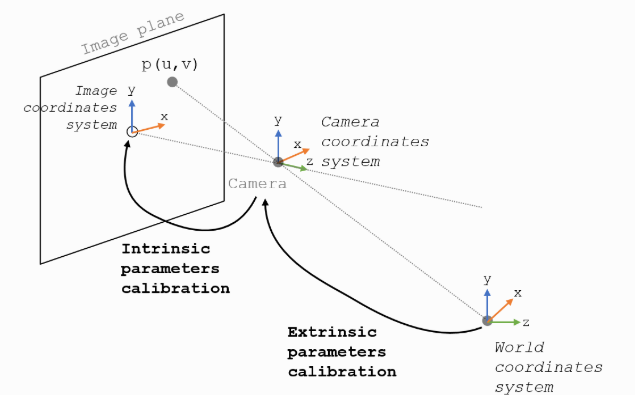
\includegraphics[width=\linewidth]{assets/background/in-extrinsic.png}
    \caption{Intrinsic and extrinsic parameter mappings \cite{mphy0026camera}}\label{fig:in-extrinsic}
  \end{subfigure}
  \hfill
  \begin{subfigure}{0.45\linewidth}
    \centering
    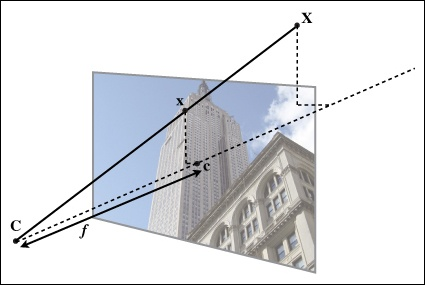
\includegraphics[width=\linewidth]{assets/background/pinhole-cam.jpg}
    \caption{Pinhole camera model \cite{solem2012programming}}\label{fig:pinhole}
  \end{subfigure}
  \caption{Camera Models}\label{fig:cam-models}
\end{figure}

\subsection {The Pin-Hole Camera}
One of the most foundational and widely used models to describe this calibration is the \emph{pin-hole} (or the  \emph{projective}) camera model \cite{solem2012programming}. 

\subsubsection{Mathematics Behind the Pin-Hole Model}
The light passes through a single point, called the camera centre, $C$, before it is projected onto the 2D image plane (giving the name pin-hole). A 3D point $\textbf{X}$ is projected onto image point $\textbf{x}$ using the equation:
\(\lambda \textbf{x} = P\textbf{X}\). where $P$ is the a 3x4 matrix called the camera (or \emph{projection}) matrix and $\textbf{X}$ is 1x4 and has four elements in homogenous coordinates, \(\textbf{X} = [x, y, z, w]\) and $\lambda$ is the inverse depth of the 3D point. Which can be needed if we want all coordinates to be homogenous with the last value ($w$) normalised to $1$.
The Camera Matrix, P can will all calibration values for the camera. So: \(P = K \left[R \mid t\right] \), $R$ is the ($3 \times 3$) rotational matrix describing the orientation of the camera, and t a ($3 \times 1$) translational vector describing the position of C.Also the intrinsic calibration matrix, K, will encode camera attributes discussed above.
\[
  K = 
  \begin{bmatrix}
    f_x & s & c_x \\
    0 & f_y & c_y \\
    0 & 0 & 1
  \end{bmatrix}
  \hspace{1cm}
  f_x = \alpha f_y
\]

Where the values are from \ref{sec:intrinsic} and $\alpha$ is the aspect ratio used for non-square pixel elements (usually safe to assume $a=1$). A simple calibration method is to use a reference object, with known dimensions $dX and dY$. Then we can measure the distance from the camera to the object $dZ$. After obtaining the image we can measure the image plane size of our object $dx, dy$ in pixels and extract the focal point as: \(
  f_x = \frac{dx}{dX} dZ , \hspace{1cm} f_y = \frac{dy}{dY}dZ
  \)Or we can use a calibration image to project and use that for calibration, see Figure \ref{fig:calin-dots}

  \begin{figure}[h]
    \centering
    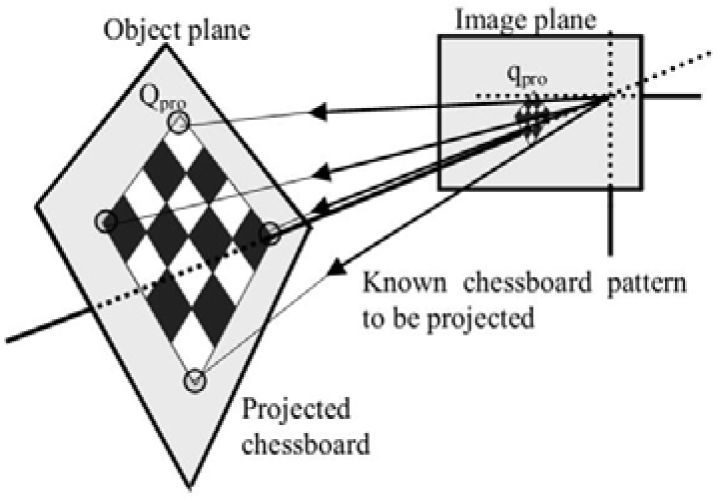
\includegraphics[width=0.4\textwidth]{assets/background/checkered.jpeg}
    \caption{Calibration pattern cite{Din2014ProjectorCalibration}}\label{fig:calin-dots}
  \end{figure}

\subsection{Other Camera Models for Robotics}
The pin-hole camera system gives us an insight into the translation of captured light into interpretable data. Although, useful for theoretical analysis, real-world cameras deviate from this idealised system quite a lot. Some camera models:
\begin{itemize}
  \itemsep0em
  \item\textbf{Different Fields of View (FOV)}
  Cameras providing different FOVs such as fish-eye or wide-angle cameras, for different degrees of vision. For example, 360-degree cameras for surveillance or autonomous driving. Where the distortion of the image must be corrected in processing.

  \item\textbf{Multiple Cameras}
  \emph{Stereo camera models} (Binocular vision) for depth measurement incorporation into the image. Two cameras which are a known distance apart can be used to perceive depth by computing the disparity between corresponding points in both images (triangulation) \cite{hamzah2016literature}. This can also be scaled to \emph{n-view stereo vision} to reduce occlusion problems while increasing redundancy in the number of viewpoints there are.\label{sec:nview}
  
  \item\textbf{Active Depth Cameras}
  These go beyond stereo vision. Such as \emph{Time-of-Flight (ToF)} cameras that emit infra-red light and measure the time it takes to reflect back, and using speed of light in calculating the depth directly \cite{foix2011tof,zanuttigh2016time}. Or \emph{structured light} cameras that project a known pattern onto a surface and observe its deformation to calculate the depth. These two are usually more concise compared to stereo vision because they offer robust depth sensing regardless of surface textures or differing lighting conditions.
  There are different lens models like the \emph{thin-lens} model which -opposing the pin-hole model- doesn't assume an infinitely small aperture. Mimicking the real world closer as cameras need lenses to focus the light. And these lenses add to the intrinsic properties of the camera.
\end{itemize}
  Therefore, choice of camera model significantly affects how a robot can perceive its environment and its calibration impacts the degree of correctness.
  
  \subsection{Visual Perception and Object Recognition}
  The goal of computer vision within robotics is to alow the robot to infer meaningful information about its surroundings and later use that information to achieve its goals. So, perception starts with understanding what is in the scene to a macro and micro level. 
  
  \subsubsection{Low-Level Vision}
    These are fundamental visual features without caring about the details of what the overlying object may be. Such as: detecting colours, corners, edges of objects. 

  \subsubsection{High-Level Vision}
    Traditional Computer Vision approaches relied on manually crafted systems to extract features from images, such as \textbf{Edge Detection:} \cite{canny1986computational, derpanis2004harris}, \textbf{Feature Descriptors:}\cite{wu2013comparative,juan2009comparison, rublee2011orb}, and \textbf{Template Matching:}\cite{brunelli2009template}.However successful these methods have been in structured settings, they don't necessarily do well with large variations in object appearance, real-world noise and dynamic backgrounds. Therefore, these can't necessarily be easily extended to work in a dynamic robotics setting.

    \subsubsection{Deep Learning-Based Approaches}
    Modern object detection and recognition is mostly reliant on deep learning methods:
    \begin{itemize}
      \item \textbf{Convolutional Neural Networks (CNNs):} These \cite{gu2018recent,li2021survey} can automatically learn hierarchical features from raw image data. Which can then be used for image classification \cite{hijazi2015using,traore2018deep}, while being robust to variations in lighting, occlusions, and perspective changes.
      \item \textbf{Region-Based CNNs (R-CNN):} These models propose candidate regions and run CNNs on that region for classifying with higher accuracy in complex scenes \cite{bharati2020deep, girshick2015fastrcnn}
      \item \textbf{Transformer Architectures (ViTs):} Recent advances in transformer architectures \cite{bi2021transformer} now being used in vision using attention mechanisms to improve object detection in cluttered environments \cite{kayacan2024vision} and be robust against long-range dependencies which CNN's suffer from due to locality of processing.
    \end{itemize}

  \subsection{Applying to Robotics}
    Despite these significant advances within Computer Vision, there are still some challenges that are present within vision in robotics that must be addressed in making a human-like dynamically learning and moving robot.

    \subsubsection{Lighting and Appearance}
      Due to expectations of robots being dynamic, they must be able to operate in varying environments where lighting and scene appearances will be constantly changes.

    \subsubsection{Occlusions}
      Within real life dynamic environments, on top of the lighting changes, object are often partially or sometimes fully occluded from where the robot might be placed or moving in the environment.  One of the simple solutions to this is to introduce multiple views for the robot. 
      
      Similar in idea to \emph{n-view} from \ref{sec:nview}, having more cameras, usually some around the scene and some on different parts of a robot (e.g. wrist-mounted, head-mounted, or mounted around the scene) allows for robustness against occlusions and introduce multiple different angles for efficiency in learning. 

      However, one big drawback is that the state space can easily explode: increasing training times and inferring speeds. On top of that, depending on the task and the robot multi-viewpoint systems might not be feasible, for example, the environment might not be as clearly defined, making the such cameras an impossibility. There are other solutions such as temporal consistency \cite{lai2018learningblindvideotemporal} which can also be extended for use in robotics, such as here \cite{billington2007using, yang2021reactive}.
      \todo[color=green]{maybe some figures here from tasks like searching drawer etc.}

      \begin{figure}[h]
        \centering
        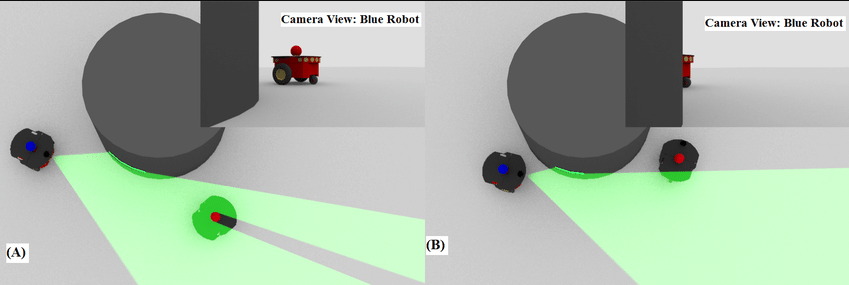
\includegraphics[width=0.7\textwidth]{assets/background/occlusion.png}
        \caption{Example of an occluded object \cite{occlusionimage}}\label{fig:occlusion}
      \end{figure}
      \todo[color=green]{better image}

    \subsubsection{Real-Time Processing}
    Another convoluted problem in vision to robotics is that, novel advancements are usually resource intensive and then scaled down once proven. Many autonomous real-time  applications such as autonomous driving, drone navigation need provably quick decision making in order to be safe to use. Therefore computational bottlenecks or unoptimised approaches requiring time and computational resources might not immediately fit into a robotics use case.

    \subsubsection{Unseen Domain Generalisations}
    Finally, another active area in robotics currently is issues such as \emph{few-shot} or even \emph{one-shot} learning, which aim to teach robots new and unseen policies with minimal new data. Or approaches such as self-supervised learning (such as here \cite{lim2022real2sim2real, huang2021robot}) to combine real and simulated data for optimising learning in new domains.
    \\\\
    One of the trajectories that can be taken in improving such static models is to take inspiration from what makes humans good visual learners. We also face issues like occlusions in day-to-day life and one advantage we have is that our vision is \textbf{active.}
    
  

    
% Active Vision 
\section{Active Vision (AV)}
    Physical robots, by actively controlling their cameras \cite{Aloimonos1988}, as well as using attention and focus mechanisms to identify the relevant parts of the environment. This, by introducing another level of decision making in the form of where and what to perceive, enables the robot to move and act more intelligently within the space provided. This approach is mostly beneficial in applications such as: autonomous navigation, multi-robot control and human-robot interactions. \cite{breazeal2001hri}
    
  \subsection{Principles of Active Vision}
  Traditional static vision enhanced by incorporating camera and viewpoint optimisations into the perception systems. Some principles include:
  \begin{itemize}
    \item \textbf{Gaze Control:} This is the fundamental idea of active vision. Move the camera and the viewpoint, (ideally) to regions of interest.
    \item \textbf{Next-Best-View Planning:} Strategically adjusting the camera to maximise the visual information the robot acquires. They often use \emph{attention mechanisms} which ensure they focus on the specific items or areas \cite{Burusa_2024} while ignoring the other cluttering information in the scene. These attention mechanisms can be \emph{spatial}, focusing on regions of interest; or \emph{temporal}: used with tracking moving objects.
    \item \textbf{Task-Driven Perception:} Optimising the visual input to the task at hand by using methods like \emph{next-best-pose} to ensure the robot stays focused on task-specific manipulations.
  \end{itemize}
  Some combinations of these fundamental ideas, fitting them to the use-case means our robot can acquire better observations of the space instead of relying on prior human knowledge to strategically pre-place the camera where it would most benefit the task, or later external manipulations, such as, researcher figuring out semi-manually where a better pose would be during testing and moving the camera between sets of tests.
  \todo{not sure if this reads as I want it}

  \subsection{Back To Markov}
  \subsubsection{Partially Observable Markov Decision 
  \label{subsec:pomdp}
  Processes (POMDPs)}
  Adding on to the definitions above in \ref{subsec:mdp}, we now require \emph{Partially Observable Markov Decision Processes (POMDPs)} 
  which is an extension of MDPs where it is defined as a 7-tuple \cite{thrun2002probabilistic,placed2023surveyactivesimultaneouslocalization}: 
  \[\langle S, A, \mathcal{Z}, \xi_S, \xi_{\mathcal{Z}}, E, \gamma \rangle \]
  
  in addition to earlier, the state transition function \( \xi_S ~\colon~ S \times A \rightarrow \Pi\left(S\right)\) and $\Pi\left(S\right)$ is the space of probability density functions (pdf) over $S$. The observation space $\mathcal{Z}$, and the conditional likelihood of making any of those observations \(\xi_{\mathcal{Z}} ~\colon~ S \rightarrow \Pi\left(Z\right)\) where $\Pi\left(\mathcal{Z}\right)$ is the space of pdfs over $\mathcal{Z}$.
  Differently to the fully observable case, agents here cannot reliably know their own true state. So, they maintain an internal \emph{belief} system (historic), $b_t\left(s_t\right)$ which represents the posterior probability over states at time $t$, given the available data collected up until that time. \(b_t\left(s_t\right) \triangleeq  \mathbb{P}\left(s_t \mid z_{1 \colon t}, a_{1 \colon t - 1}\right)\) where the given is the history, $h$.
  \\\\
  Introducing this belief system we can now model active tasks which rely on exploring the space for the optimal states and selecting an action that decreases the uncertainty in the belief state, leading to actively informed decision-making.

  \todo{MAYBE? note on synchronoous and asynchronous active vision from the "observe then act" paper}

  \subsection{Active Vision in Practice}
  There are a number of ways to implement active vision in practice. Some common methods are:

  \subsubsection{RL for Active Perception}
    Framing this problem as a decision-making one, so: ``Where should the agent face to maximise reward'' allows us to come up with a policy which can learn where to look next, optimise the pose of the camera to minimise uncertainty in decisions and adapt to different environments \cite{rothbucher2011,zhangembodied}. Which can then be modelled as a POMDP system and solved as classical RL, giving us a way to control the gaze during a tasks execution.

  \subsubsection{Predictive Control}
  Instead of allowing random exploration of the viewpoint space we can also train models that predict the next best view using techniques such as Entropy-based viewpoint selection and Bayesian optimisations with the use of prior information such as the knowledge of the scene, object models' geometry and symmetries \cite{dhami2023prednbvpredictionguidednextbestview3d,breyer2022closedloopnextbestviewplanningtargetdriven}
  \\\\
  With these implementation strategies we can use active learning for tasks such as:
  \begin{itemize}
    \item \textbf{Dexterous manipulation robots} (i.e. grasping robots), where a eye-in-hand camera (maybe) coupled with depth sensing can refine its understanding of its surroundings and actively adjust views to avoid occlusions. 
    \item \textbf{Autonomous navigation,} mobile robots can use approaches like Active SLAM \cite{} \todo{find the active SLAM paper again}, to map their environments and refine their understanding of it constantly. Some examples may be aerial drones continuously exploring and learning more about different regions \cite{}.
    \item \textbf{Human-robot interactions,} social robots can be made to keep eye contact or learn to track human mannerisms from gestures and expressions to make them more realistic in interactions.
  \end{itemize}
    
  \subsection{Challenges}
  Despite all the discussed possibilities, Active Vision still remains fairly theoretical and unexplored compared to other areas of robotics. Although, the ideas have been floating around in computing circles for almost three decades, there are several challenges that need to be overcome for active vision to be viable for all its possible applications.
  \begin{enumerate}
    \item \textbf{Computational Complexity:}
    \item \textbf{Sensor, Hardware and Environmental Limitations:}
    \item \textbf{Integrations with other Sensing Mediums:}
    \todo{complete this section}
  \end{enumerate}

  \todo{write the connecting bit here that transitions us to related work}
